%%
%% This is file `mcmthesis-demo.tex',
%% generated with the docstrip utility.
%%
%% The original source files were:
%%
%% mcmthesis.dtx  (with options: `demo')
%% 
%% -----------------------------------
%% 
%% This is a generated file.
%% 
%% Copyright (C)
%%     2010 -- 2015    by Zhaoli Wang
%%     2014 -- present by Liam Huang
%% 
%% This work may be distributed and/or modified under the
%% conditions of the LaTeX Project Public License, either version 1.3
%% of this license or (at your option) any later version.
%% The latest version of this license is in
%%   http://www.latex-project.org/lppl.txt
%% and version 1.3 or later is part of all distributions of LaTeX
%% version 2005/12/01 or later.
%% 
%% This work has the LPPL maintenance status `maintained'.
%% 
%% The Current Maintainer of this work is Liam Huang.
%% 
\documentclass{mcmthesis}
\mcmsetup{CTeX = false,   % 使用 CTeX 套装时,设置为 true
        tcn = 2001560, problem = C,
        sheet = true, titleinsheet = true, keywordsinsheet = false,
        titlepage = false, abstract = true}
\usepackage{palatino}
\usepackage{lipsum}

% \title{A Wealth of Data}
% \author{\small \href{http://www.latexstudio.net/}
%   {
\includegraphics[width=7cm]{mcmthesis-logo}}}
\date{\today}

\usepackage{geometry}
\geometry{left=1in,right=0.75in,top=1in,bottom=1in}
\usepackage{lastpage}

%%%%%%%%%%%%%%%%%%%%%%%%%%%%%%%%%%%%%%%%
\newcommand{\Problem}{C}    % 换成你的题号
\newcommand{\Team}{2001560} % 换成你的队号
%%%%%%%%%%%%%%%%%%%%%%%%%%%%%%%%%%%%%%%%

\begin{document}

\thispagestyle{empty}
\vspace*{-16ex}
\centerline{\begin{tabular}{*3{c}}
	\parbox[t]{0.3\linewidth}{\begin{center}\textbf{Problem Chosen}\\ \Large \textcolor{red}{\Problem}\end{center}}
	& \parbox[t]{0.3\linewidth}{\begin{center}\textbf{2020\\ MCM/ICM\\ Summary Sheet}\end{center}}
	& \parbox[t]{0.3\linewidth}{\begin{center}\textbf{Team Control Number}\\ \Large \textcolor{red}{\Team}\end{center}}	\\
	\hline
\end{tabular}}
%%%%%%%%%%% Begin Summary %%%%%%%%%%%

\vspace{2em}
\begin{center}
\Large\bf Title of you paper   % 论文标题
\end{center}

From here, begin your summary  % 摘要

%%%%%%%%%%% End Summary %%%%%%%%%%%

\clearpage
\pagestyle{fancy}
% Uncomment the next line to generate a Table of Contents
%\tableofcontents 
\newpage
\setcounter{page}{1}
\rhead{Page \thepage\ of \pageref{LastPage}}

\tableofcontents
\newpage

% \begin{abstract}
%   \lipsum[1]
% \end{abstract}
% \maketitle
%%
%% Generate the Memorandum, if it's needed.
\memoto{Marketing Director of Sunshine Company}
\memofrom{MCM Team \#2001560}
\memosubject{Special Online Sales Strategy for Sunshine Company}
\memodate{\today}
% \logo{\LARGE I'm pretending to be a LOGO!}
\begin{memo}[Letter]
Dear Marketing Director,
\\\\
Thank you for your trust in our team. We have learned that you want to start with ratings and reviews and get some relevant parameters or metrics to quantify the reputation of the product, thereby increasing product attractiveness and sales. After a thorough study, we have built a model that analyze the synthesize evaluation of products to help you identify the reputation of the products and whether they are successful in the online market.
\\\\
After analyzing the data, we found that we cannot evaluate the quality and reputation of a product based on star ratings only. Because not only the star rating and the content of the review do not match well, there are some cases where non-purchasers make biased reviews of the product. These problematic stars and reviews can mislead customers, affect their shopping decisions, affect future review trends, and even damage product reputation.
\\\\
Firstly, we removed reviews from non-purchasers(Amazon Vine members are identified as purchasers) from the data, which minimizes the potential for malicious reviewers to damage the reputation of the product. 
\\\\
Then, we studied each review through TD-IDF (information retrieval and data mining technology) to analyze the term frequency and give each review a sentiment score, which indicates the actual semantics. By coefficient simulation, We found that there has a strong correlation between the stars and sentiment score while some are not fitting well, which shows that star rating and sentiment score both modify the quality of the product.
\\\\
We suppose there is a distinction between product reputation and product quality for various quality reviews can have diverse effects on product reputation. A single word 'Perfect' is inadequate, while a detailed description of the praise brings more forward message to the customer. Amazon Vine member reviews and reviews with high ratings are credible.We established a review quality score model to value the review. When the star rating and the sentiment score are similar, the quality is more top; when the star rating and the review sentiment score do not harmonize, the quality is lower.
\\\\
By synthesize evaluation model, we take word length, helpfulness rate, whether it is from a vine member and review quality score and sentiment score into consideration to define the synthesize evaluation score, which represents a product's reputation.
\\\\
When your products are on the online market, by examining the synthesize evaluation score over time, you can discern whether the products are potentially fruitful. Through analyzing the three types of products' synthesize evaluation score, we list several reasons for the changes in product reputation in a certain period. They assists you to pay attention to some particular breakpoints to optimize listing in time and improve the product reputation.
\begin{itemize}
	\item A specific review may incite customers to write positive or negative reviews. You need to have an eye on negative reviews and appropriately invite customers to write reviews that benefit the product reputation.

	\item Poor overall review quality (inconsistent star ratings and review content) may cause product reputation to decline.

	\item Inviting more Amazon Vine Members to write reviews can improve the product reputation.

	\item When multiple bad reviews with high quality appear, not only estimating the negative impact of these reviews is necessary, but also pay attention to the shortcomings of products, and feedback these opinions to the design manufacturers to improve the products.
\end{itemize}
We sincerely hope that it will provide you with useful information. Wish very best wished for your job and your products!
\\\\
Team \#2001560

\end{memo}

\section{ Introduction }
\subsection{Background}
In recent years, quantities of customers prefer shopping online for its less spacetime limitation and the convenient home delivery service. However, compared to the traditional physical stores, customers can only evaluate products by the provided profile and pictures instead of seeing or testing the real ones. The information gap here is one of the leading causes of dissatisfied purchases. To help customers know the product better, many online marketplace platforms, such as Amazon, launch a "review system". Customers can express their level of satisfaction and further opinions or information about purchases through rating and reviewing. That additional information can help not only other customers make purchasing decisions, but companies improve the pros and cons of product design.\\

However, we found that not all reviews are equally relevant. Some reviews are too general; some people's ratings do not match their reviews; there are even deliberately misleading reviews, such as malicious defamation from competitors or the raise by the bribed reviewers. Therefore, when using data to assist business decisions, we need to analyze data carefully and comprehensively to obtain more accurate results. More factors should be considered, such as the ratings, review contents, and review time, rather than straightly calculate the average rating level.

\subsection{Problem Restatement}
Analyze the three product data sets to describe quantitative and/or qualitative patterns, relationships that help evaluate a product's star ratings, reviews, and helpfulness ratings. Use data to demonstrate that they are valuable.\\

Solve the following issues through modeling:
\begin{itemize}
  \item Determine the most informative metric based on ratings and reviews. This metric can track the product ratings of three products when they are on the market.
  
  \item Analyze the relationship between product ratings and time in three data sets.
  
  \item Look for critical factors that can affect the inflection point of product ratings through time.
  
  \item Analyze whether there will be more a series of positive or negative reviews over a while and whether customer star ratings will be affected by recent reviews.
  
  \item Whether star rating and the keyword of review content match.
\end{itemize}

\subsection{ Data }
\subsubsection{Data Source}
Our model is informed by the customer-supplied ratings and reviews for microwave ovens, baby pacifiers, and hair dryers sold in the Amazon marketplace over more than ten years.
\subsubsection{Data Pre-processing}
We did the following to sanitize the data set:
\begin{itemize}
  \item Remove factors that were not measured at all, such as marketplace and product category, for they can not present any information.
  
  \item Remove the redundant factors, such as review\_id and product\_id, for they can be completely replaced by customer\_id and product\_parent.
  
  \item Remove factors that could mislead the model, such as verify\_purchase==N while vine==N.
  
  \item Remove some garbled character.
\end{itemize}

\section{ Assumptions }
\begin{itemize}
  \item Merchant's purpose: Guide users to buy products with quality reviews and recent reviews.
\end{itemize}
\begin{itemize}
  \item The content of the review and the star rating should be the same. People believe in reviews when review content is inconsistent with star ratings.

Reason: Based on popular psychology, real language is convincing 
\end{itemize}
\begin{itemize}
  \item Amazon Vine members' reviews are credible, excluding subjective factors that give high ratings for free products.

Reason: Big data select Amazon Vine members. Their evaluations are more objective and practical.
\end{itemize}
\begin{itemize}
  \item Actual purchasers' reviews are credible.

Reason: People who have already experienced the product know more about the actual performance of the product.
\end{itemize}
\begin{itemize}
  \item Comments from actual non-purchasers (except Amazon Vine members) are untrustworthy.

Reason: Amazon provides Amazon Vine members with free copies of the product. Hence Amazon Vine members should be identified as purchasers. We listed the distribution of 1-5 stars between the non-purchasers and the purchasers. It shows that the non-purchasers give more 1 star than purchasers, which may mislead the reviews.

- fig1+2 Compare the non-purchasers with the purchasers on star rating.
\end{itemize}
\begin{itemize}
  \item The impact of the same purchaser on reviews is not taken into consideration; that is, each evaluation behaviour of the purchaser is independent and not related to the previous reviews.
\end{itemize}

\section{Nomenclature}
\begin{table}[h]
  \centering
  \begin{tabular}{ccc}
    \hline
    Symbol & Definition\\
    \hline
    star$_{i}$ & star rating of a review i\\
    
    ER$_{i}$ & emtional rating of a review i\\
      
    d$_{i}$ & the variance between star rating and emtional rating of a review i\\

    L$_{i}$ & length of a review i\\

    Vm$_{i}$ & whether a review i is from an Amazon vine member\\
      
    Vr$_{i}$ & votes rating of a review i\\
      
    M$_{i}$ & rating of a review i\\

    Q$_{i}$ & quality of a review i\\
          
    R$_{i}$ & synthesize evaluation of a review i\\
    
    R & average review synthesize evaluation\\
      
    t & time\\
    \hline
  \end{tabular}
  \caption{variables and functions}
\end{table}

\section{ Model Design }

\section{ Part \uppercase\expandafter{\romannumeral1}:  Rating Model based on star-ratings and reviews}

\section{ Part \uppercase\expandafter{\romannumeral2}:  Synthesize Evaluation Model}

\section{ Solution }

\section{ Sensitivity Analysis }

\section{ Strengths and Weaknesses }
\subsection{Strengths}
\begin{itemize}
  \item \textbf{Applies widely}\\
        This  system can be used for many types of airplanes, and it also
        solves the interference during  the procedure of the boarding
        airplane,as described above we can get to the  optimization
        boarding time.We also know that all the service is automate.
  \item \textbf{Improve the quality of the airport service}\\
        Balancing the cost of the cost and the benefit, it will bring in
        more convenient  for airport and passengers.It also saves many
        human resources for the airline. \item \textbf{}
\end{itemize}
\subsection{Weaknesses and Improvement}
\begin{itemize}
  \item Due to the lack of sufficient data, the parameters used in the model are mainly obtained through actual life experience and repeated adjustment experiments. It would be profitable if we could get further data which can objectively reflect the quality of reviews or product quality, such as reviews with a more significant number of votes, or product sales data. By using these data, we are capable of performing a regression analysis on the model to obtain more accurate coefficients.
\end{itemize}
\begin{itemize}
  \item The LDA model has an excellent performance with document collection, while the majority of reviews are short in words. 
\end{itemize}
\begin{itemize}
  \item While major reviewers are not Amazon Vine Member, different people may have different criteria for evaluation, which may produce an objective assessment. We need to study every reviewers' rating habit to get a weight for every reviewer.
\end{itemize}
\begin{itemize}
  \item Removing the non-purchasers' reviews helps analysis the problem; however, these overt reviews may hurt the customers' purchasing decisions and further ratings.
\end{itemize}

\section{Conclusions}

\begin{figure}[h]
  \small
  \centering
  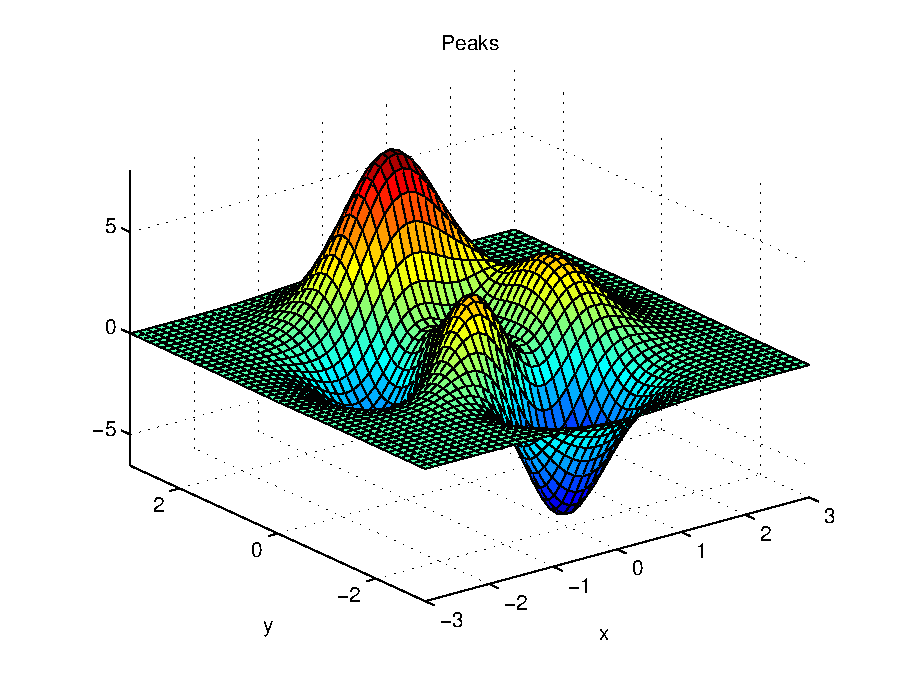
\includegraphics[width=12cm]{mcmthesis-aaa.eps}
  \caption{aa} \label{fig:aa}
\end{figure}

\lipsum[8] \eqref{aa}
\begin{equation}
  a^2 \label{aa}
\end{equation}


\[
  p_{j}=\begin{cases} 0,              & \text{if $j$ is odd}  \\
    r!\,(-1)^{j/2}, & \text{if $j$ is even}
  \end{cases}
\]

%% References
\begin{thebibliography}{99}
  \bibitem{1} D.~E. KNUTH   The \TeX{}book  the American
  Mathematical Society and Addison-Wesley
  Publishing Company , 1984-1986.
  \bibitem{2}Lamport, Leslie,  \LaTeX{}: `` A Document Preparation System '',
  Addison-Wesley Publishing Company, 1986.
  \bibitem{3}\url{http://www.latexstudio.net/}
  \bibitem{4}\url{http://www.chinatex.org/}
\end{thebibliography}

\begin{appendices}

  \section{First appendix}

  \lipsum[13]

  Here are simulation programmes we used in our model as follow.\\

  \textbf{\textcolor[rgb]{0.98,0.00,0.00}{Input matlab source:}}
  \lstinputlisting[language=Matlab]{./code/mcmthesis-matlab1.m}

  \section{Second appendix}

  some more text \textcolor[rgb]{0.98,0.00,0.00}{\textbf{Input C++ source:}}
  \lstinputlisting[language=C++]{./code/mcmthesis-sudoku.cpp}

\end{appendices}
\end{document}

%% 
%% This work consists of these files mcmthesis.dtx,
%%                                   figures/ and
%%                                   code/,
%% and the derived files             mcmthesis.cls,
%%                                   mcmthesis-demo.tex,
%%                                   README,
%%                                   LICENSE,
%%                                   mcmthesis.pdf and
%%                                   mcmthesis-demo.pdf.
%%
%% End of file `mcmthesis-demo.tex'.
